% !TeX root = ../main.tex

\chapter{石墨烯的导电性及其应用}
\section{石墨烯的导电性}


依靠紧束缚模型可以计算出石墨烯的能带分布。在紧束缚模型中电子想要跃迁到其他地方,需要脱离原子的势场,所以我们在分析一个原子附近的电子受到的作用时,认为受该原子势场的作用为主,其他原子势场的作用看成微扰,就可以得到能带分布。石墨烯的能带分布图如下。

\begin{figure}[H]
  \centering
  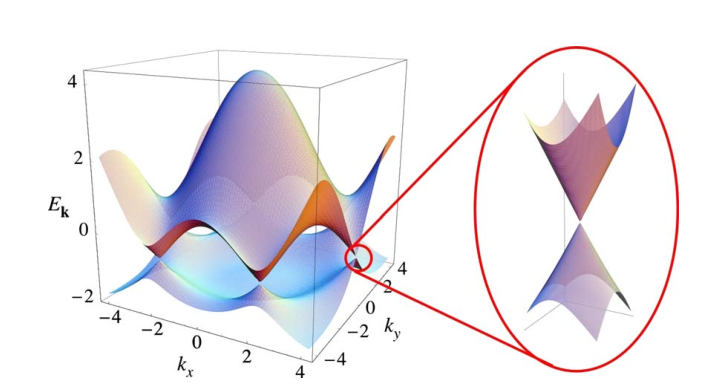
\includegraphics[scale=0.8]{img/石墨烯的能带分布,右边是狄拉克点附近.png}
  \caption{石墨烯的能带分布,右边是狄拉克点附近}
  \label{fig:grapheneDiracPoint}
\end{figure}

在$K$,$K'$点附近,我们能得到附近波矢$k=K+q$的色散关系,$E_{\pm} (q)\approx \pm \frac{3ta}{2} \left | q \right | + O\left [(q/K)^{2}  \right ]$,是近似线性的。动量与能量的关系为线性,因此电子的速度为常量,记$v_F=\frac{3ta}{2}$。

描述电子运动时,我们可以把一个在晶格内运动的电子等效为一个在自由空间中运动的电子。类似地引入有效质量的概念,将晶体中的场对于电子的影响等效于自由空间运动的电子的质量$\frac{1}{m_*}\sim \frac{d^{2}E}{dk^2}$,由于色散关系为线性,且在能量为零的点对称,导致$E(k)$在$K$点不连续,导致二阶导数无穷大,所以电子的有效质量为零。故用薛定谔方程来描述粒子的运动已无效,应该运用引入了相对论效应的狄拉克方程来描述。

事实上当我们将电子算符在$K$,$K’$进行傅里叶展开,代入哈密顿量之后,我们可以得到一个与二维的无质量电子的狄拉克方程近似的方程:

\begin{equation}
  % \label{...}
  iv_{F}\sigma \cdot \nabla \psi(r)=E \nabla (r)
\end{equation}

波函数在$K$的分量为:

\begin{equation}
  \phi_{\pm,K}(k) = \dfrac 1 {\sqrt {2}} \left(\begin{array}{c}
      -i\theta/2         \\
      \pm e^{i\theta /2} \\
    \end{array}\right)
\end{equation}
在$K'$的分量为:

\begin{equation}
  \phi_{\pm,K^{\prime}}(k) = \dfrac 1 {\sqrt {2}} \left(\begin{array}{c}
      i\theta/2           \\
      \pm e^{-i\theta /2} \\
    \end{array}\right)
\end{equation}

将$M$作为原点,两个分量的方向轴对称,且相位差为$\pi$,粒子波函数在两个波矢方向的分量可以等效为一组自旋量。螺旋度是动量算子对于自旋方向的投影,螺旋度的算子定义为$\hat{h} =\frac{1}{2} \sigma \cdot \frac{p}{\left | p \right | }  $。由于自旋量是粒子的波函数的动量分量,所以其螺旋度为$\pm 1/2$。这与狄拉克方程中所描述的无质量的自旋为$\pm 1/2$的电子相似,狄拉克方程中,正离子自旋方向只会与动量方向相同,反粒子自旋方向与动量方向相反,而在石墨烯中$K$,$K'$附近的电子就对应的是正粒子,空穴对应的是反粒子。这样电子与空穴与狄拉克方程所描述自由空间中无质量的两种状态的电子等效,所以可把石墨烯狄拉克的空穴与电子称为狄拉克费米子,$K$,$K'$被称为狄拉克点。

空穴与电子也可以在能量为零的点相互转化,且不消耗能量,因此若改变石墨烯纵向的电压,可以得到不同种类和浓度的载流子

关于石墨烯非常高的电子迁移率的原因也是由于狄拉克点的存在,由于量子隧穿效应的影响,电子有概率穿过高于自身能量的势场,对于如下图的势场,通过计算我们可以得到狄拉克费米子的隧穿概率:

\begin{equation}\label{...}
  T(\phi )\simeq \frac{cos^{2}\phi }{1-cos^{2}(Dq_{x})sin^{2} \phi }
\end{equation}

$\phi$趋于$0$时概率趋于$1$,这意味着石墨烯中的电子和空穴有较长的自由程,电子运动受温度影响较小。石墨烯有很高的电子迁移率。

以上说明石墨烯有良好的导电性。


\section{石墨烯导电性的应用}
\subsection{超级电容器}
超级电容器是是介于电容器和电池之间的储能器件,是传递能量和储存能量的体系。石墨烯的比表面积非常大而且导电性能优异,使得电子的聚集能力提高且扫面电压稳定。使用石墨烯作为电极大大减少了充电时间而且容量提高了$5-6$倍。

\begin{figure}[H]
  \centering
  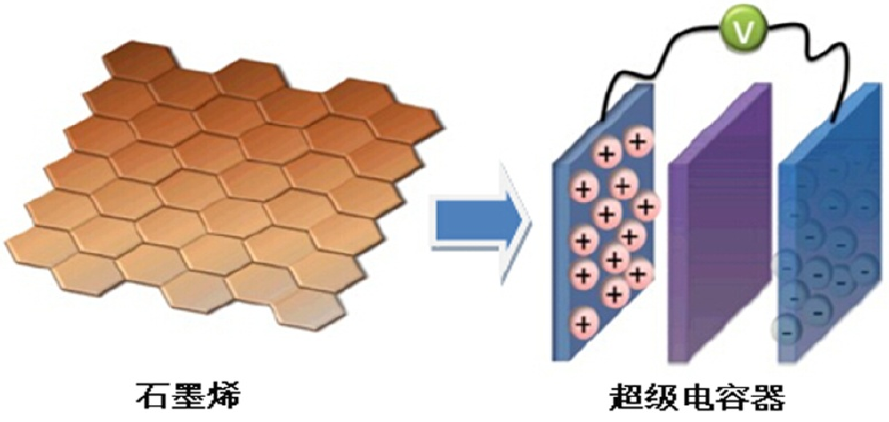
\includegraphics[scale=0.8]{img/石墨烯用于超级电容器的电极材料.png}
  \caption{石墨烯用于超级电容器的电极材料}
\end{figure}

Stoller等人使用单层石墨烯作为超级电容器的电极,分别在水中比电容为$135F/g$ 和在有机电解液中比电容为$99F/g$。Le等人使用的新的方法将石墨烯溶液直接喷墨打印在钛网上,然后通过热还原法制备出石墨烯薄膜的超级电容器。经过伏安法扫描$1000 $次后,比电容从$ 125F/g $下降到$121F/g$,损失率不到 $3\%$。Ning 等人用模板化学沉积法制备可控结构的石墨烯网,石墨烯网厚度有 $1-2$ 层,比表面积有$1654m^{2}/g$。将石墨烯网作为超级电容器电极在KOH 溶液中测试比电容达到$245F/g$ 同时 $2000$ 次伏安循环后还保持在 $94.1\%$。制备的基于石墨烯的平面结构的超级电容器,质量比电容可以达到$250F/g$,面积比电容高于以前的报道达到了$394F/cm^{2}$。

基于石墨烯的超级电容器方面具有非常大的应用潜力。目前就提高石墨烯比表面积和导电性,还有较大的突破空间。\cite{wangqingkai}


\subsection{石墨烯在锂离子电池中的应用}
石墨烯因具有巨大的比表面积、优异的电性能和稳定的化学性能,目前已被广泛应用于锂离子电池的负极材料中。锂离子电池的负极主要作为储锂的主体,石墨烯既具备提供良好电子传输通道的能力,又有优异的锂离子传输性能,故能提升传输性能。Yoo等采用氧化还原法制备得到石墨烯,并将其应用于锂离子电池负极材料,实验数据显示,首次循环的比容量有明显提升,比容量值可达$540 mAh/g$。

石墨烯在二维高比表面积上具备特殊结构,因此被应用于锂离子电池的正极材料中。该项特点使电子的传输能力得到进一步提升,从而对正极材料的导电性能进行全面改善,并提升了锂离子的传输能力。目前的研究表明,石墨烯与LiFePO$_{4}$、LiNi$_{1/3}$Co$_{1/3}$Mn$_{1/3}$O$_{2}$和LiMn$_{2}$O$_{4}$等复合形成的复合正极材料可提升材料的电化学性能。\cite{kejiahan}


\subsection{石墨烯在防腐涂料的应用}
石墨烯薄膜能贴附在金属表面,将金属与氧气、水等隔绝,加入到原有的涂料中,使得涂料表面的空隙减小,加强隔绝性能;石墨烯机械性能良好,掺入防腐涂料后形成迷宫状结构,具有优异的弹性和抗变形能力;石墨烯具有优良导电性,可以采用电化学防腐。故石墨烯在防腐涂料领域广泛应用。

石墨烯在防腐涂料的应用分为石墨烯薄膜、石墨烯功能化修饰、石墨烯填料。
石墨烯薄膜很难被腐蚀,能够对被贴附的材料进行有效的保护,例如石墨烯掺杂量为$0.4\%$时,能够将聚酰胺涂层的摩擦寿命提高$880\%$。功能化修饰例如以乙二胺与氧化石墨烯表面的羧基发生脱水缩合反应,制得纳米氧化石墨烯(NGO,Nano Graphene Oxide)。之后以NGO作为填料,加入到环氧树脂涂料中,制备得到复合防腐涂料。以石墨烯做环氧树脂涂料的填料可以有效地增强环氧树脂涂料的耐腐蚀能力、力学性能,延长使用寿命。\cite{lifei}

